\documentclass{report}

\usepackage{textcomp}
\usepackage{graphicx}
\usepackage{fancyhdr}
\usepackage{subcaption}
\usepackage{multicol}
\usepackage{outlines}
%===================================
\newcommand{\classinfo}{{\bf Basic ACL \\ Configuration}\\{\it CIT 167}\\{Chaz Davis}}
\newcommand{\semester}{BCTC \\ Spring 2020}
%===================================
\newcommand{\mysection}[1]{\section*{#1}}
\newcommand{\mysubsection}[2]{\textbf{\romannumeral #1) #2}}
%===================================
\setlength{\headheight}{15.2pt}
\pagestyle{fancy}
\fancyhf{}
\lhead{ \fancyplain{}{Chaz Davis} }
\rhead{ \fancyplain{}{\today} }
\cfoot{ \fancyplain{}{\thepage} }
\renewcommand{\headrulewidth}{0.5pt}
\renewcommand{\footrulewidth}{0pt}

%===================================
\title{\classinfo}
\author{\semester}
\date{\today}

%===================================

\begin{document}

\maketitle

%===================================
\mysection{\textbf{Part 1: Configuring the Network}}

\mysubsection{1}{Configuring the PCs}\\
I set up the devices according to the diagram. I then configured the PCs
according to the diagram. You can see in Fig.~\ref{Conf17}
on Pg.~\pageref{Conf17}.


Next, I configured the Router, you can see the output of 
{\scriptsize{\verb$show ip int brief$}\normalsize} in You can see in
Fig.~\ref{Conf17}\subref{Conf17R1} 
on Pg.~\pageref{Conf17}.

\begin{figure}[!hbt]\centering
\subfloat[IP Configuration of Joes PC]{\label{Conf17PC1}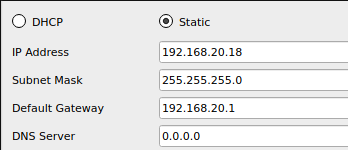
\includegraphics[width=.45\linewidth]{Figures/JoeIpConfig.png}}\hfill
\subfloat[IP Configuration of Susans PC]{\label{Conf17PC2}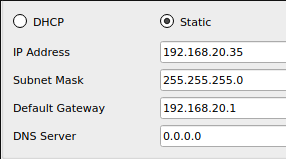
\includegraphics[width=.45\linewidth]{Figures/SusanIPConfig.png}}\par 
\subfloat[IP Configuration of Williams PC]{\label{Conf17PC3}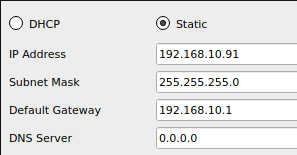
\includegraphics[width=.45\linewidth]{Figures/WilliamIpConfig.png}}\hfill
\subfloat[Show Ip int brief on R1]{\label{Conf17R1}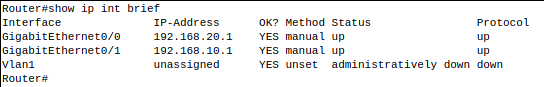
\includegraphics[width=.45\linewidth]{Figures/R1Config.png}}\par
\caption{IP Configuration of the PCs on the network}\label{Conf17}
\end{figure}

\noindent\mysubsection{2}{Verifying the Network}\\
Next, I used the pcs to ping the other PCs on the network. The output of which
can be seen in You can see in Fig.~\ref{Net17}\subref{Net17Ping1} through
Fig.~\ref{Net17}\subref{Net17Ping4}
on Pg.~\pageref{Net17}.



\begin{figure}[!hbt]\centering
\subfloat[William pinging Joe's PC]{\label{Net17Ping1}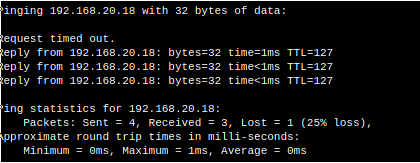
\includegraphics[width=.45\linewidth]{Figures/WilliamPingingJoe.png}}\hfill
\subfloat[William Pinging Susan's PC]{\label{Net17Ping2}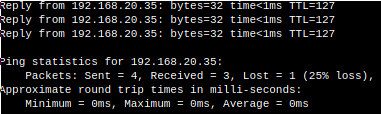
\includegraphics[width=.45\linewidth]{Figures/WilliamPinginSusan.png}}\par
\subfloat[Susan pinging William's PC]{\label{Net17Ping3}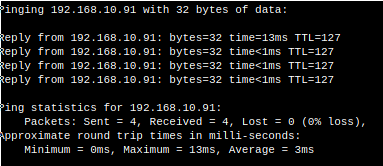
\includegraphics[width=.45\linewidth]{Figures/SusanPingingWilliam1.png}}\hfill
\subfloat[Joe pingin Williams PC]{\label{Net17Ping4}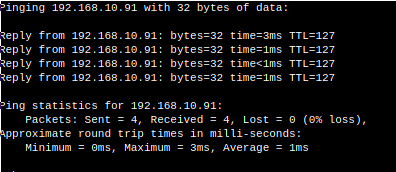
\includegraphics[width=.45\linewidth]{Figures/JoePingingWilliam1.png}}\par
\caption{Router and PC's configured on the network}\label{Net17}
\end{figure}


\noindent\mysubsection{3}{Creating and applying the standard ACL}\\
I set up a standard ACL named PERMIT-JOE, with the following lines
{\scriptsize{\verb$10 permit host 192.168.20.18$}\normalsize} 

{\scriptsize{\verb$20 deny any$}\normalsize} 
You can see in Fig.~\ref{acl17}~\subref{acl17pj1}.


Next, I applied that to int g0/1 as an outgoing
acl (Fig.~\ref{acl17}\subref{acl17pj2})

Finally, I verified that it had been applied correctly to the router, see
Fig.~\ref{acl17}\subref{acl17pj3} and Fig.~\ref{acl17}\subref{acl17pj4} on
Pg.~\pageref{acl17}.

\begin{figure}[!hbt]\centering
\subfloat[creating PERMIT-JOE acl]{\label{acl17pj1}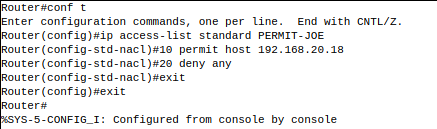
\includegraphics[width=.45\linewidth]{Figures/ConfiguringPermitJoe.png}}\hfill
\subfloat[Applying PERMIT-JOE acl]{\label{acl17pj2}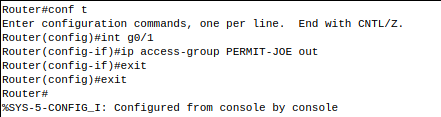
\includegraphics[width=.45\linewidth]{Figures/ApplyingPermitJoe.png}}\par
\subfloat[Output of show ip int]{\label{acl17pj3}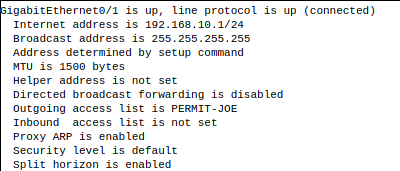
\includegraphics[width=.45\linewidth]{Figures/ShowIpIntPermitJoe.png}}\hfill
\subfloat[output of show run]{\label{acl17pj4}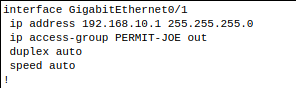
\includegraphics[width=.45\linewidth]{Figures/ShowRunPermitJoe.png}}\par
\caption{Configuring and applying PERMIT-JOE}\label{acl17}
\end{figure}



\noindent\mysubsection{4}{Verifying the ACL is working}\\
I attempted to ping William's PC from
Joe (Fig.~\ref{Verify17}\subref{Verify17Ping1}), this was successful.
I then, attempted to ping William's PC from
Susan (Fig.~\ref{Verify17}\subref{VerVerify17Ping2}), this was unsuccessful.


\begin{figure}[!hbt]\centering
\subfloat[Joe Pinging William's PC]{\label{Verify17Ping1}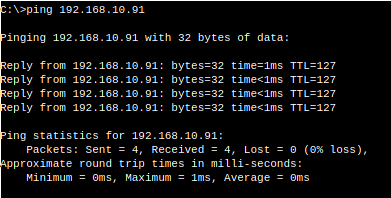
\includegraphics[width=.45\linewidth]{Figures/JoePinginWilliam2.png}}\hfill
\subfloat[Susan attempting to ping William's PC]{\label{Verify17Ping2}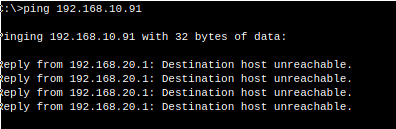
\includegraphics[width=.45\linewidth]{Figures/SusanPingingWilliam2.png}}\par 
\caption{Successfully applied ACL PERMIT-JOE}\label{Verify17}
\end{figure}




\noindent\mysubsection{2}{Creating and Applying An ACL}\\
In order to block all traffic from the 192.168.10.0 Network, I would create and
inbound acl on g0/1 that says 
{\scriptsize{\verb$10 deny 192.168.10.0 0.0.0.255$}\normalsize} 
I could also create a deny any on that same inbound port, as thats the only
netowrk on that port, but as other networks can be created in the future, I
feel like that would be the safest way to go about this.
%===================================

\end{document}
